\documentclass[11pt]{article}
\usepackage{geometry}                
\geometry{letterpaper}                 
\usepackage[parfill]{parskip}        
\usepackage{graphicx}
\usepackage{amssymb}
\usepackage{amsmath}
\usepackage{epstopdf}
\usepackage{verbatim}
\usepackage{float}
\usepackage{enumerate}
\usepackage{hyperref}
\usepackage[utf8]{inputenc}
\usepackage[T1]{fontenc}
\DeclareGraphicsRule{.tif}{png}{.png}{`convert #1 `dirname #1`/`basename #1 .tif`.png}
\usepackage{color}
\usepackage{textcomp}
\definecolor{listinggray}{gray}{0.9}
\definecolor{lbcolor}{rgb}{1,1,1}


\begin{document}
Solution for problem 4.53 from O\&S, problem \#5 on hmwk 6

\section*{(a)}

If $X(e^{j\omega })$ and $H_0(e^{j\omega })$ are as shown in Figure P4.53-2, sketch (to within a scale factor) $X_0(e^{j\omega })$, $G_0(e^{j\omega })$, $Y_0(e^{j\omega })$.

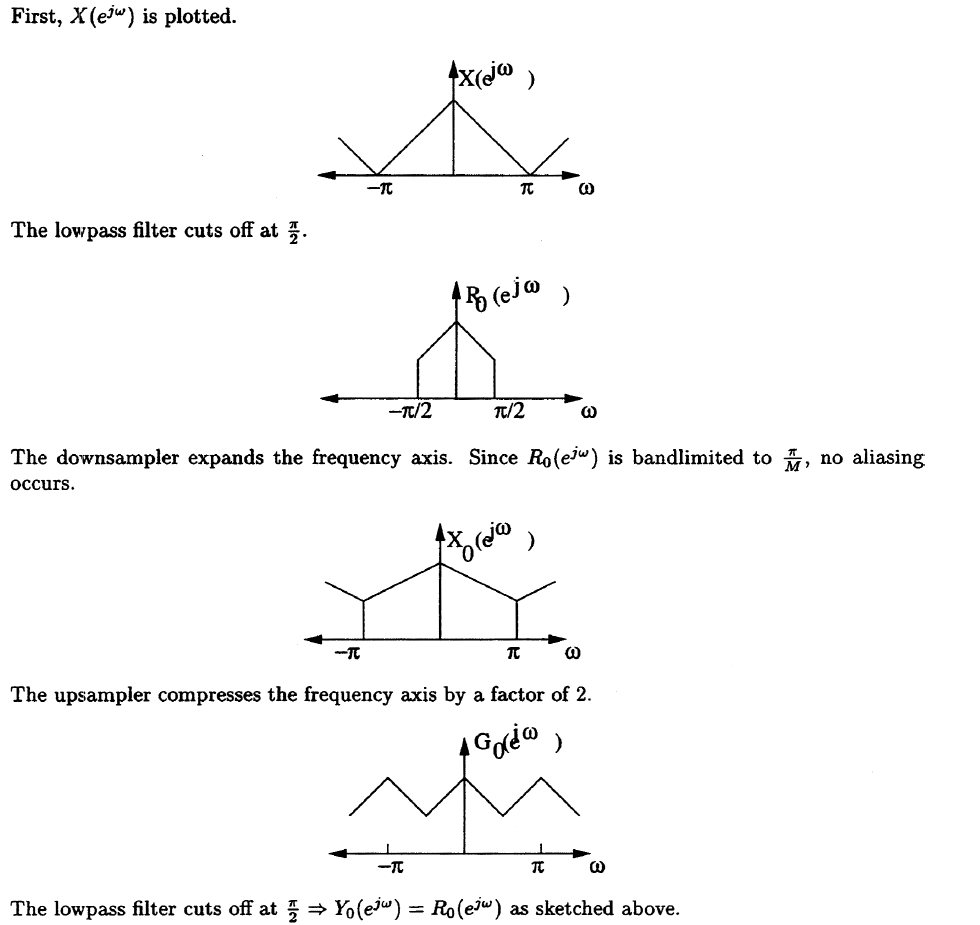
\includegraphics[width=\textwidth]{hmwk6_p5_a.png} 

\section*{(b)}
Write a general expression for $G_0(e^{j\omega })$ in terms of $X(e^{j\omega })$ and $H_0(e^{j\omega })$. Do \textit{not} assume that $X(e^{j\omega })$ and $H_0(e^{j\omega })$ are as shown in Figure 4.53-2.

\begin{eqnarray*}
R_0(e^{j\omega }) &=& X(e^{j\omega })H_0(e^{j\omega }) \\
X_0(e^{j\omega }) &=& \frac{1}{2}\left(R_0\left(e^{j\frac{\omega}{2}}\right)+R_0\left(e^{j\left(\frac{\omega}{2}-\pi\right) }\right) \right) \\
G_0(e^{j\omega}) &=& X_0(e^{j2\omega}) \\
&& \text{So combining these together...} \\
X_0(e^{j\omega}) &=& \frac{1}{2}\left(X_0\left(e^{j\frac{\omega}{2}}\right)H_0\left(e^{j\frac{\omega}{2}}\right)+X_0\left(e^{j\left(\frac{\omega}{2}-\pi\right) }\right) H_0\left(e^{j\left(\frac{\omega}{2}-\pi\right) }\right)\right) \\
G_0(e^{j\omega}) &=& \frac{1}{2}\left(X_0\left(e^{j\omega}\right)H_0\left(e^{j\omega}\right)+X_0\left(e^{j\left(\omega-\pi\right) }\right) H_0\left(e^{j\left(\omega-\pi\right) }\right)\right) \\
\end{eqnarray*}

\section*{(c)}
Determine a set of conditions on $H_0(e^{j\omega })$ that is as general as possible and that will guarantee that $y[n]$ is proportional to $x[n-n_d]$ for any stable input $x[n]$.

NOTE: If you have a particular version of 2nd edition, the wording is different: $|Y(e^{j \omega})| \propto |X(e^{j \omega})|$. The final reconstruction is also a difference rather than a sum: $y[n] = y_0[n]-y_1[n]$. This will be discussed at the end.

\begin{eqnarray*}
Y_0(e^{j\omega}) &=& H_0(e^{j\omega})G_0(e^{j\omega}) \\
&=& \frac{1}{2}X(e^{j\omega})H_0^2(e^{j\omega})+X(e^{j(\omega-\pi)})H_0(e^{j\omega})H_0(e^{j(\omega-\pi)}) \\ 
\text{Similarly, } && \\
Y_1(e^{j\omega}) &=& \frac{1}{2}X(e^{j\omega})H_1^2(e^{j\omega})+X(e^{j(\omega-\pi)})H_1(e^{j\omega})H_1(e^{j(\omega-\pi)}) \\ 
Y(e^{j\omega}) &=& Y_0(e^{j\omega}) + Y_1(e^{j\omega}) \\
&=& \frac{1}{2}X(e^{j\omega})\left[H_0^2(e^{j\omega})+H_1^2(e^{j\omega}) \right]+\frac{1}{2}X(e^{j(\omega-\pi)}) \left[H_0(e^{j\omega})H_0(e^{j(\omega-\pi)})+H_1(e^{j\omega})H_1(e^{j(\omega-\pi)}) \right]\\
\end{eqnarray*}

Using the given relationship that $H_1(e^{j\omega}) = H_0(e^{j(\omega-\pi)})$,

\begin{eqnarray*}
Y(e^{j\omega}) &=& \frac{1}{2}X(e^{j\omega})\left[H_0^2(e^{j\omega})+H_0^2(e^{j(\omega-\pi)}) \right]+\frac{1}{2}X(e^{j(\omega-\pi)}) \left[H_0(e^{j\omega})H_0(e^{j(\omega-\pi)})+H_0(e^{j(\omega-\pi)})H_0(e^{j\omega}) \right]\\
&=& \frac{1}{2}X(e^{j\omega})\underbrace{\left[H_0^2(e^{j\omega})+H_0^2(e^{j(\omega-\pi)}) \right]}_{A(\omega)}+ X(e^{j(\omega-\pi)}) \underbrace{\left[H_0(e^{j\omega})H_0(e^{j(\omega-\pi)}) \right]}_{B(\omega)}\\
\end{eqnarray*}

Our goal is to have $y[n] \propto x[n-n_d]$, or in the frequency domain, $Y(e^{j\omega}) = c e^{j\omega n_d}X(e^{j\omega})$. Note that this is the same as the 3rd edition wording because $|Y(e^{j \omega})| = |c e^{j\omega n_d}X(e^{j\omega}) | = |c|\cdot |X(e^{j \omega})|$. Thus, we want the aliasing term $X(e^{j(\omega-\pi)})$ to go away completely. Therefore we choose $B(\omega) = 0,\ \forall \omega$. Additionally, we desire to have $A(\omega) = c e^{j\omega n_d}$.

\subsection*{Analyzing $B(\omega)$}

Supposing we have $H_0(e^{j\omega})$ with lower cutoff frequency $\omega_L$ and upper cutoff frequency $\omega_R$, then $B(\omega) = 0,\ \forall \omega$ can be enforced if $ H_0(e^{j\omega})$ and $H_0(e^{j(\omega-\pi)}) $ do not overlap, i.e. $\pi + \omega_L > \omega_R$. Rearranging terms we have $\pi > -\omega_L+\omega_R$, or the width of the low-pass filter must be less than $\pi$.

\subsection*{Analyzing $A(\omega)$}

\subsubsection*{Case 1: $n_d = 0$}

For case of $n_d = 0$, our goal simplifies to $Y(e^{j\omega}) = c X(e^{j\omega})$, so we want $A(\omega) = c_1$, some constant $c_1$, for all $\{\omega | X(e^{j \omega}) \neq 0\}$ (the support of $X(e^{j \omega})$). However, to make this system general for all signals (even ones that aren't bandlimited), let us say that $A(\omega) = c_1 \ \forall \omega$.

\begin{eqnarray*}
H_0^2(e^{j\omega})+H_0^2(e^{j(\omega-\pi)}) &=& c_1 \\
\end{eqnarray*}

Combined with the fact that $ B(\omega)=0$, 
\begin{eqnarray*}
H_0^2(e^{j\omega}) &=& c_1,\ \omega \in \{\omega_L,\omega_R\} \\
H_0^2(e^{j(\omega-\pi)}) &=& c_1,\ \omega \in \{\pi+\omega_L,\pi+\omega_R\} \text{ redundant, so I will drop this line of reasoning}\\
H_0(e^{j\omega}) &=& \sqrt{c_1},\ \omega \in \{\omega_L,\omega_R\} \\
\end{eqnarray*}

Choosing $c_1 = 2c$, we satisfy the necessary condition. Therefore, $H_0(e^{j\omega})$ should have constant height over its support and zero phase. This is equivalent to an ideal low pass filter.

\subsubsection*{Case 2: $n_d \neq 0$}

For the case of $n_d \neq 0$, 
\begin{eqnarray*}
\frac{1}{2}\left[ H_0^2(e^{j\omega})+H_0^2(e^{j(\omega-\pi)}) \right] &=& c e^{j \omega n_d} \\
\frac{1}{2}\left[|H_0(e^{j\omega})|e^{j\angle H_0(e^{j\omega})} \right]^2 + \frac{1}{2}\left[|H_0(e^{j(\omega-\pi)})|e^{j\angle H_0(e^{j(\omega - \pi)})} \right]^2 &=& c e^{j \omega n_d} \\
\frac{1}{2}|H_0(e^{j\omega})|^2 e^{2j\angle H_0(e^{j\omega})} + \frac{1}{2}|H_0(e^{j(\omega-\pi)})|^2 e^{2j\angle H_0(e^{j(\omega - \pi)})}  &=& c e^{j \omega n_d} \\
\end{eqnarray*}

Now we consider two cases: (a) $\omega \in \{\omega_L, \omega_R\}$ (in the support of $H_0(e^{j\omega})$) and (b) $\omega > \omega_R$ or $\omega < \omega_L$ (in the support of $H_0(e^{j(\omega-\pi)})$.

\subsubsection*{Case 2a}

For $\omega \in \{\omega_L, \omega_R\}$, $H_0(e^{j(\omega-\pi)})= 0$, so 

\begin{eqnarray*}
\frac{1}{2}|H_0(e^{j\omega})|^2 e^{j2\angle H_0(e^{j\omega})}  &=& c e^{j \omega n_d} \\
\frac{1}{2}|H_0(e^{j\omega})|^2 &=& c \quad \rightarrow \quad |H_0(e^{j\omega})| = \sqrt{2c}\\
e^{j2\angle H_0(e^{j\omega})}  &=& e^{j \omega n_d} \quad \rightarrow \quad \angle H_0(e^{j\omega}) = \frac{1}{2} \omega n_d \\
\end{eqnarray*}

In other words, $H_0(e^{j\omega})$ must have constant magnitude and linear phase.

\subsubsection*{Case 2b}

For $\omega \not\in \{\omega_L, \omega_R\}$, $H_0(e^{j\omega})= 0$, so 

\begin{eqnarray*}
\frac{1}{2}|H_0(e^{j(\omega-\pi)})|^2 e^{j2\angle H_0(e^{j(\omega-\pi)})}  &=& c e^{j \omega n_d} \\
\frac{1}{2}|H_0(e^{j(\omega-\pi)})|^2 &=& c \quad \rightarrow \quad |H_0(e^{j(\omega-\pi)})| = \sqrt{2c}\\
e^{j2\angle H_0(e^{j(\omega-\pi)})}  &=& e^{j \omega n_d} \quad \rightarrow \quad \angle H_0(e^{j(\omega-\pi)}) = \frac{1}{2} \omega n_d \\
\end{eqnarray*}

Thus, we see that when shifted $H_0(e^{j\omega})$ should still have constant magnitude (which is consistent with what we saw in case 2a). We also see that the phase of shifted $H_0(e^{j\omega})$ is the same as the phase of unshifted $H_0(e^{j\omega})$. This implies that the phase is periodic with period $\pi$.

Thus our final conditions for $H_0(e^{j\omega})$ are that:

 $|H_0(e^{j\omega})| = \sqrt{2c}$ 
 
and 

$\angle H_0(e^{j\omega}) = \begin{cases}
\frac{1}{2} \omega n_d, & \omega \in \{\omega_L,\omega_R \} \\
\frac{1}{2} (\omega-\pi) n_d, & \omega \in \{\pi+\omega_L,\pi+\omega_R \}
\end{cases}$. 

Note that if we choose $n_d = 0$, this reduces to our previous conditions. 

\subsection*{Alternate version of problem}
For the particular version of the 2nd edition/3rd edition:

\begin{eqnarray*}
Y(e^{j\omega}) &=& Y_0(e^{j\omega}) - Y_1(e^{j\omega}) \\
&=& \frac{1}{2}X(e^{j\omega})\left[H_0^2(e^{j\omega})-H_1^2(e^{j\omega}) \right]+\frac{1}{2}X(e^{j(\omega-\pi)}) \left[H_0(e^{j\omega})H_0(e^{j(\omega-\pi)})-H_1(e^{j\omega})H_1(e^{j(\omega-\pi)}) \right]\\
\end{eqnarray*}

Using the given relationship that $H_1(e^{j\omega}) = H_0(e^{j(\omega-\pi)})$,

\begin{eqnarray*}
Y(e^{j\omega}) &=& \frac{1}{2}X(e^{j\omega})\left[H_0^2(e^{j\omega})-H_0^2(e^{j(\omega-\pi)}) \right]+\frac{1}{2}X(e^{j(\omega-\pi)}) \left[H_0(e^{j\omega})H_0(e^{j(\omega-\pi)})-H_0(e^{j(\omega-\pi)})H_0(e^{j\omega}) \right]\\
&=& \frac{1}{2}X(e^{j\omega})\underbrace{\left[H_0^2(e^{j\omega})+H_0^2(e^{j(\omega-\pi)}) \right]}_{A(\omega)}\\
\end{eqnarray*}

We desire $|Y(e^{j\omega})| \propto |X(e^{j\omega})|$, so 

\begin{eqnarray*}
|Y(e^{j\omega})| &=& c |X(e^{j\omega})| \\
|\frac{1}{2}X(e^{j\omega})A(\omega)|&=& c |X(e^{j\omega})| \\
\frac{1}{2}|X(e^{j\omega})|\cdot |A(\omega)|&=& c |X(e^{j\omega})| \\
|A(\omega)| = 2c \\
\end{eqnarray*}

So long as $A(\omega) = H_0^2(e^{j\omega})+H_0^2(e^{j(\omega-\pi)})$ has constant magnitude, we have $|Y(e^{j\omega})| \propto |X(e^{j\omega})|$. Note that in this version of the problem, we do not have the requirement that $H_0(e^{j\omega})$ not overlap with $H_0(e^{j(\omega-\pi)})$.

\subsection*{Note to graders}

Since this problem was different depending the students' textbooks, please be aware that if they had the alternate version of the problem ($y[n]=y_0[n]-y_1[n]$), they should have completed the analysis in the above section for full credit. If they had the first version of the problem ($y[n]=y_0[n]+y_1[n]$), they need to have completed the analysis at least for the $n_d=0$ case. Any additional analysis is optional.

\end{document}